%% 
%% Copyright 2007, 2008, 2009 Elsevier Ltd
%% 
%% This file is part of the 'Elsarticle Bundle'.
%% ---------------------------------------------
%% 
%% It may be distributed under the conditions of the LaTeX Project Public
%% License, either version 1.2 of this license or (at your option) any
%% later version.  The latest version of this license is in
%%    http://www.latex-project.org/lppl.txt
%% and version 1.2 or later is part of all distributions of LaTeX
%% version 1999/12/01 or later.
%% 
%% The list of all files belonging to the 'Elsarticle Bundle' is
%% given in the file `manifest.txt'.
%% 

%% Template article for Elsevier's document class `elsarticle'
%% with numbered style bibliographic references
%% SP 2008/03/01

% \documentclass[preprint,12pt]{elsarticle}
\documentclass[preprint,12pt,authoryear]{elsarticle}


%% Use the option review to obtain double line spacing
%% \documentclass[authoryear,preprint,review,12pt]{elsarticle}

%% Use the options 1p,twocolumn; 3p; 3p,twocolumn; 5p; or 5p,twocolumn
%% for a journal layout:
%% \documentclass[final,1p,times]{elsarticle}
%% \documentclass[final,1p,times,twocolumn]{elsarticle}
%% \documentclass[final,3p,times]{elsarticle}
%% \documentclass[final,3p,times,twocolumn]{elsarticle}
%% \documentclass[final,5p,times]{elsarticle}
%% \documentclass[final,5p,times,twocolumn]{elsarticle}

%% For including figures, graphicx.sty has been loaded in
%% elsarticle.cls. If you prefer to use the old commands
%% please give \usepackage{epsfig}

%% The amssymb package provides various useful mathematical symbols
\usepackage{amssymb}
\usepackage{pslatex}
\usepackage{newtxmath}
\usepackage{graphicx}
\usepackage{color,soul}
\usepackage[normalem]{ulem}
%\usepackage{epstopdf}
\usepackage{subcaption}

%% The amsthm package provides extended theorem environments
%% \usepackage{amsthm}

%% The lineno packages adds line numbers. Start line numbering with
%% \begin{linenumbers}, end it with \end{linenumbers}. Or switch it on
%% for the whole article with \linenumbers.
%% \usepackage{lineno}

\journal{Biologically Inspired Cognitive Architecture}

\begin{document}

\begin{frontmatter}

%% Title, authors and addresses

%% use the tnoteref command within \title for footnotes;
%% use the tnotetext command for theassociated footnote;
%% use the fnref command within \author or \address for footnotes;
%% use the fntext command for theassociated footnote;
%% use the corref command within \author for corresponding author footnotes;
%% use the cortext command for theassociated footnote;
%% use the ead command for the email address,
%% and the form \ead[url] for the home page:
%% \title{Title\tnoteref{label1}}
%% \tnotetext[label1]{}
%% \author{Name\corref{cor1}\fnref{label2}}
%% \ead{email address}
%% \ead[url]{home page}
%% \fntext[label2]{}
%% \cortext[cor1]{}4554edsxi
%% \address{Address\fnref{label3}}
%% \fntext[label3]{}

\title{Lateral Inhibition: Essential Component of Temporal Difference Learning}

%% use optional labels to link authors explicitly to addresses:
%% \author[label1,label2]{}
%% \address[label1]{}
%% \address[label2]{}

\author{{\large \bf Jacob Rafati \& David C.~Noelle} \\
        {\large \bf (jrafatiheravi@ucmerced.edu, dnoelle@ucmerced.edu)} \\
        Computational Cognitive Neuroscience Laboratory \\
        University of California, Merced}

\address{5200 North Lake Road \\
        Merced, CA 95343 USA}

\begin{abstract}
%% Text of abstract
There is growing support for Temporal Difference (TD) Learning as a
formal account of the role of the midbrain dopamine system and the
basal ganglia in learning from reinforcement. This account is
challenged, however, by the fact that realistic implementations of TD
Learning have been shown to fail on some fairly simple learning tasks
--- tasks well within the capabilities of humans and non-human
animals. We hypothesize that such failures do not arise from natural
learning systems because of the ubiquitous appearance of lateral
inhibition in the cortex, producing sparse conjunctive internal
representations that support the learning of predictions of future
reward. We provide support for this conjecture through computational
simulations that compare TD Learning systems with and without lateral
inhibition, demonstrating the benefits of sparse conjunctive codes for
reinforcement learning.
\end{abstract}

\begin{keyword}
%% keywords here, in the form: keyword \sep keyword

%% PACS codes here, in the form: \PACS code \sep code

%% MSC codes here, in the form: \MSC code \sep code
%% or \MSC[2008] code \sep code (2000 is the default)
Reinforcement learning; lateral inhibition; sparse conjunctive codes;
computational cognitive neuroscience.

\end{keyword}

\end{frontmatter}

%% \linenumbers

%% main text

%%Introduction
\section{Introduction}
\label{sec:introduction}

% Inspiration from biology to show that TD RL with a VFA can solve difficult problems if lateral inhibition is used to produce sparse internal representations of the state
Humans and non-human animals are capable of learning highly complex
skills by reinforcing appropriate behaviors with reward. The midbrain
dopamine system has long been implicated in reward-based
learning~\citep{SchultzW:1993:Dopamine}, and the information processing
role of dopamine in learning has been well described by a class of
reinforcement learning algorithms called \emph{Temporal Difference
(TD) 
Learning}~\citep{MontaguePR:1996:Dopamine,SchultzW:1997:Science}. While 
TD Learning, by itself, certainly does not explain all observed
reinforcement learning phenomena, increasing evidence suggests
that it is key to the brain's adaptive
nature~\citep{DayanP:2008:Ugly}.

Beyond empirical support for the TD Learning account of biological
reinforcement learning, the power of this learning method suggests
that it may be capable of explaining the neural basis of the
successful learning of even fairly complex
tasks~\citep{SuttonRS:1998:Book}. This algorithm can learn
elaborate decision making skills, such as playing the game of
Backgammon at the Grand Master
level~\citep{TesauroG:1995:TDGammon}. There are even proofs that TD
Learning will converge to optimal performance, given enough
experience~\citep{DayanP:1992:Proof}.

Despite these strengths, a mystery remains. There are some relatively
simple reinforcement learning problems for which TD Learning has been
shown to fail~\citep{Boyan:1995:Approximating}. These problems arise
when the space of possible sensory states of the learning agent is so
large that it is intractable to store the agent's learned assessment
of the \emph{value} or \emph{quality} of each state (i.e., its
expectation of future reward, given that it is in that state) in a
large look-up table. In these cases, it is necessary to encode the
agent's learned \emph{value function}, mapping from sensory state
features to an expectation of future reward, using some form of
function approximator. Formally, this function approximator is a
parameterized equation that maps from state to value, where the
parameters can be constructively optimized based on the experiences of
the agent. One common function approximator is an artificial neural
network, with the parameters being the connection weights in the
network. Such a network, adapted using the \emph{backpropagation of
error} learning method~\citep{RumelhartDE:1986:BP}, was used in the
previously mentioned Backgammon playing
program~\citep{TesauroG:1995:TDGammon}. As illustrated by this program,
TD Learning with an artificial neural network approximating the value
function, can solve apparently complex tasks. Using a function
approximator to learn the value function has the added benefit of
potentially supporting generalization by including a bias toward
mapping similar sensory states to similar predictions of future
reward.

Surprisingly, some tasks that superficially appear very simple cannot
be perfectly mastered using this method. For example, learning to
navigate to a goal location in a simple two-dimensional space in which
there are obstacles has been shown to pose a substantial challenge to
TD Learning using a backpropagation neural
network~\citep{Boyan:1995:Approximating}. Note that the proofs of
convergence to optimal performance depend on the agent maintaining a
potentially highly discontinuous value function in the form of a large
look-up table, so the use of a function approximator for the value
function violates the assumptions of those formal analyses. Still, it
seems unusual that this approach to learning can succeed at some
difficult tasks but fail at some fairly easy tasks.

The power of TD Learning to explain biological reinforcement learning
is greatly reduced by this observation. If TD Learning fails at simple
tasks that are well within the reach of humans and non-human animals,
then it cannot be used to explain how the dopamine system supports
such learning.

In this paper, we demonstrate how incorporating a ubiquitous feature
of biological neural networks into the artificial neural networks used
to approximate the value function can allow TD Learning to succeed at
simple tasks that have previously challenged it. Specifically, we show
that the incorporation of \emph{lateral inhibition}, producing
competition between neurons so as to produce \emph{sparse conjunctive
representations}, can produce success in learning to approximate the
value function using an artificial neural network, where only failure
had been previously found. Thus, through computational simulation, we
provide preliminary evidence that lateral inhibition in the brain may
help compensate for a weakness of TD Learning, further buttressing the
TD Learning account of dopamine-based reinforcement learning.

In the remainder of this paper, we initially provide some background
concerning the reported failure of TD Learning on fairly simple
problems. We then provide details concerning our computational
simulations of TD Learning with lateral inhibition included. The
results of these simulations, comparing the performance of our
approach to previously examined methods, are then described. We close
with a discussion of these results and ideas for future work.


% section introduction (end)

% Background
\section{Background} % (fold)
\label{sec:background}
% Temporal Difference Learning ... Actor/Critic Architecture
\subsection{Temporal Difference Learning} % (fold)
\label{sub:temporal_difference_learning}
Reinforcement Learning consist of four main elements: a set of world states; a set of actions available at each state for the agent; a transition function, which is the probablity of transision from a state to another state performing an specific action; and a reward function, which is the corresponding reward or cost for such a transition \citep{SuttonRS:1998:Book,Botvinick-Niv-Barto:2009:HRL}. The RL agent in actor-critic implemention is devided to two main modules, the actor, which is responsible to select action based on a modifiablie policy and adptive critic which maintains state-action values. The policy function is a mapping from percieved states of envirionment to the actions to be taken by the RL agent and the action-state value fucntion is the stimates of expected cumulative future reward (or cost) for any state-action pair. During agent's experience of the task, the action-selection policy $\pi(s)$  and state-action values $Q(s,a)$ modify based on the feedback from environment in terms of reward signal (from fixed critic) to reach the optimum policy or behaviour (see Figure \ref{fig:TD-schematic}).   

\begin{figure}
\begin{subfigure}{.5\textwidth}
  \centering
  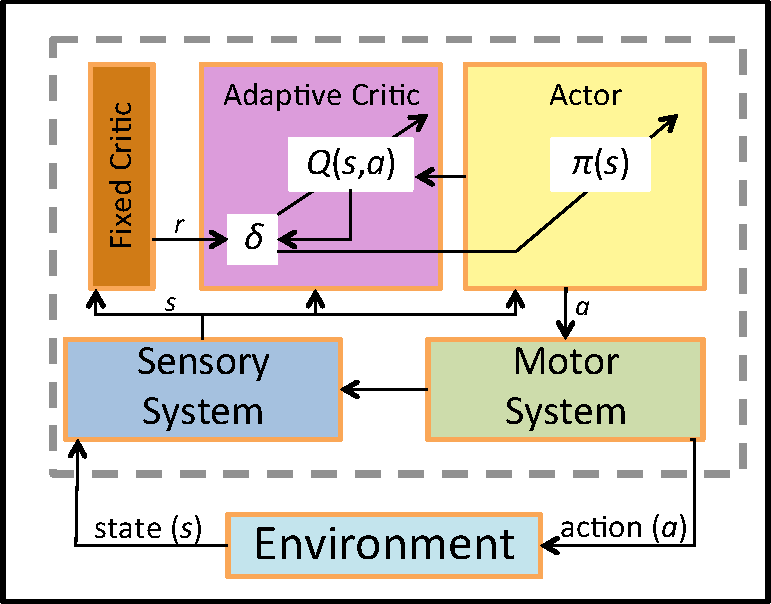
\includegraphics[width=.8\linewidth]{figures/TD-comp-model-schematic.pdf}
  \caption{}
  \label{fig-sub:actor-critic-schematic}
\end{subfigure}%
\begin{subfigure}{.5\textwidth}
  \centering
  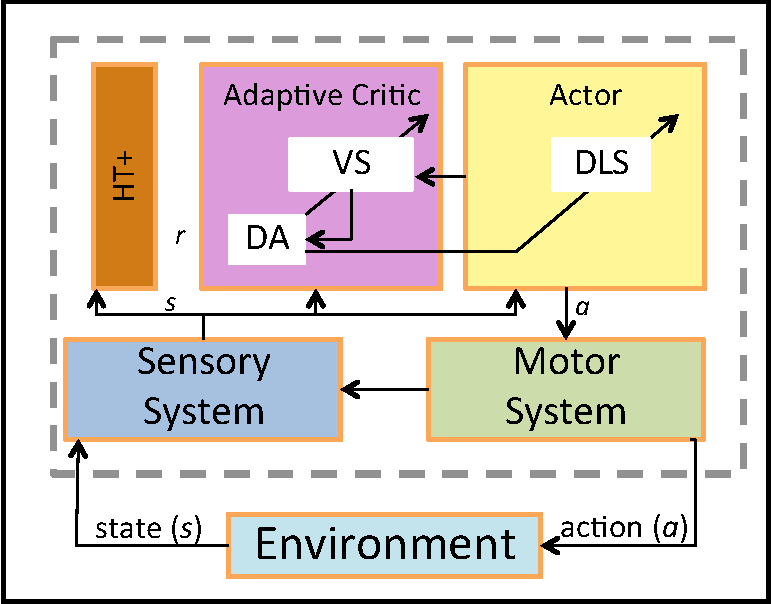
\includegraphics[width=.8\linewidth]{figures/TD-brain-schematic.pdf}
  \caption{}
  \label{fig-sub:actor-critic-brain-schematic}
\end{subfigure}
\caption{An actor-critic RL. (a) Schematic of the RL actor–critic model structure. $r$: reward signal; $Q(s,a)$: state-action value function; $\delta$: temporal- difference prediction error; $\pi(s)$: policy function. (b) An actor-critic model of brain. \emph{VS}: ventral Striatum, \emph{DLS}: dorso-lateral Striatum, \emph{DA}: dopamine, \emph{HT+}: Hypothalamus.}
 \label{fig:TD-schematic}
\end{figure}

Consider a very simple two-dimensional ``grid world'' environment that
remains static over time. A reinforcement learning agent in this
environment may be faced with the choice, at each time step, to move a
fixed distance either North, South, East, or West. On each time step,
the agent receives mild negative reinforcement, until it moves to a
goal location in the Northeast corner of the space, at which point the
agent is relieved of negative reinforcement. Further, imagine that
this environment contains ``puddles'' through which the agent can
move, but moving into puddle locations produces extremely strong
negative reinforcement. Finally, consider the case in which the agent
can perfectly sense its location in the grid environment (i.e., its
Cartesian coordinates), but it otherwise has no senses. This situation
is illustrated in Figure~\ref{puddleworld}. Equipped with TD Learning,
using a function approximator to learn the value function, could such
an agent learn to avoid the puddles and move rapidly to the goal
location, after substantial experience in the environment?

\begin{figure}
\begin{center}
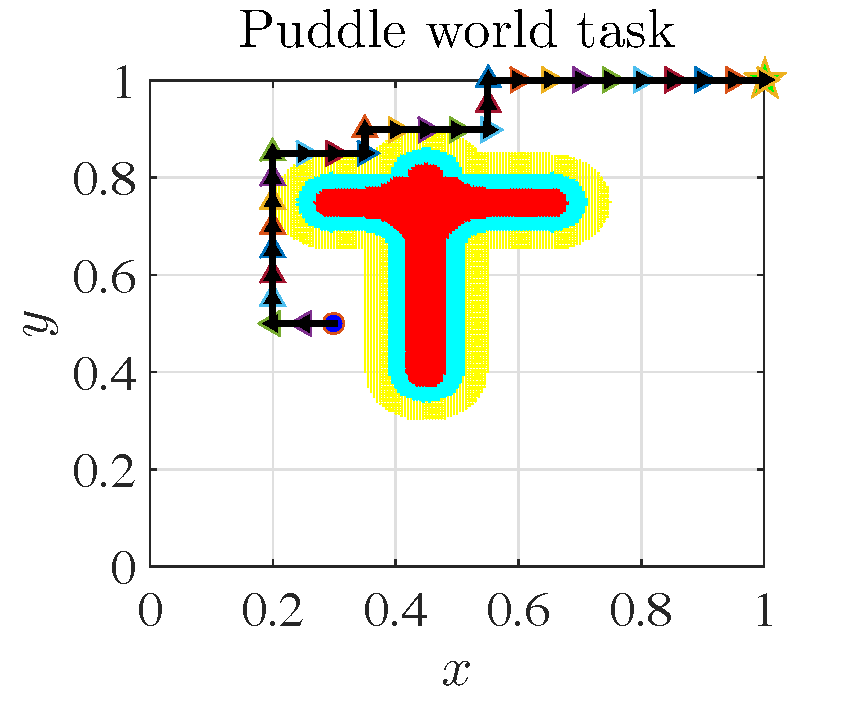
\includegraphics[scale=0.5]{figures/puddleworld.pdf}
\end{center}
\vspace{-4mm}
\caption{The agent receives $-1$ reward on each time step until it
         reaches the goal in the Northeast corner. The agent moves a
         distance of $0.05$ either North, South, East, or West on each
         time step. Entering a puddle produces a reward of $(-400
         \times d)$, where $d$ is the shortest distance to a puddle
         edge.}
\label{puddleworld}
\end{figure}

% Boyan & Moore
% Sutton - carefully engineered for the problem (especially Acrobat)
% kWTA ... O'Reilly & Munakata (2000) .... O'Reilly Neural Computation

\cite{Boyan:1995:Approximating} provided simulation evidence
suggesting that such learning is impossible. They tried a variety of
different value function approximators, including a backpropagation
network with a single hidden layer, but none of them converged on a
good solution to the problem. Indeed, as the agent continued to
explore the environment, the estimate of future reward for locations
kept changing, failing to settle down to a fixed value function.

This observation suggests that the difficulty in learning this problem
arises from a specific feature of reinforcement learning. In
particular, the value function that the function approximator is
trying to learn is, in a way, a moving target. Early in training, when
the agent is unlikely to make it to the goal location, the expected
future reward for a given location might be quite low. Later, if the
agent has had some successes, the value for the same location might be
higher. If the value function is stored in a large look-up table, then
adjusting the value of one location has no influence on the values
associated with other locations, allowing for small incremental
changes in the value function. When using a function approximator,
however, adjusting parameters (e.g., backpropagation network
connection weights) for one location will likely change the value
assigned to many other locations, potentially causing the un-learning
of appropriate values for those other locations. This is a reasonable
hypothesis for the observed lack of convergence.

In the following year, \cite{SuttonRS:1996:Coarse} showed that this
task could be learned by a TD Learning agent by hard-wiring the hidden
layer units of the backpropagation network used to learn the value
function to implement a fixed sparse conjunctive (coarse) code of the
agent's location. The specific encoding used was one that had been
previously proposed in the CMAC model of the
cerebellum~\cite{AlbusJS:1975:CMAC}. Each hidden unit would become
active only when the agent was in a location within a particular range
of $x$ values \emph{and} within a particular range of $y$ values. The
conjoining of conditions on both coordinates is what made this code
``conjunctive'' in nature. Also, for any given location, only a small
fraction of the hidden units displayed non-zero activity. This is what
it means for the hidden representation to be a ``sparse''
code. Locations that were close to each other in the environment
produced more overlap in the hidden units that were active than
locations that were separated by a large distance. By ensuring that
most hidden units had zero activity when connection weights were
changed, this approach kept changes to the value function in one
location from having a broad impact on the expected future reward at
distant locations. (In the backpropagation of error learning
algorithm, a connection weight is changed in proportion to the
activity on the sending side of that connection, so there is no change
if there is no activity being sent.) By engineering the hidden layer
representation, this reinforcement learning problem was solved.

This is not a general solution, however. If the same approach was
taken for another reinforcement learning problem, it is quite possible
that the CMAC representation would not be appropriate. Thus, the
method proposed by \cite{SuttonRS:1996:Coarse} does not help us
understand how TD Learning might flexibly learn a variety of
reinforcement learning tasks. This approach requires prior knowledge
of the kinds of internal representations of sensory state that are
easily associated with expected future reward, and there are simple
learning problems for which such prior knowledge is unavailable.

We hypothesize that the key feature of the
\citep{SuttonRS:1996:Coarse} approach is that it produces a sparse
conjunctive code of the sensory state. Representations of this kind
need not be fixed, however, but might be learned at the hidden layers
of neural networks. Computational cognitive neuroscience models have
shown that a combination of feedforward and feedback inhibition
naturally produces sparse conjunctive codes over a collection of
excitatory neurons~\citep{OReillyRC:2001:CECN}. Such patterns of
lateral inhibition are ubiquitous in the mammalian
cortex~\citep{KandelE:2012:Book}. Importantly, networks containing such
lateral inhibition can still learn to represent input information in
different ways for different tasks~\citep{OReillyRC:2001:CECN},
retaining flexibility while producing the kind of sparse conjunctive
codes that may support reinforcement learning.




% subsection temporal_difference_mechanism (end)

%Boyan and Moore \citep{Boyan:1995:Approximating}  are training their function approximator over a finite set of sampled states. In each iteration of their Smooth Value iteration the function approximator is not been trained for the states wwhich the agent is experiencing but for the entire sampled states and this can be probelmatic when dealing with a nonlinear dynamic control problems that they are presenting in their work. Sutton is called thsi method of generalization as offline learnign which is not quite accurate. So the failure of artifitial neural network in their work is because of the algorithm of set of training. Their function approximator will remain passive for the states which are not included in the sampled set. They treated the function approximator as a ``smoothing function'' rather than using as ``active learner''. Their algorithm doesn't involve exploration. 
% section background (end)

%%Experimental Design
\section{Experimental Design} % (fold)
\label{sec:experimental_design}
% State Encoding
% Determining Optimal Value Functions (Q Table)
% Linear AC
% Backpropagation AC
% kWTA AC


In order to assess our hypothesis that biasing a neural network toward
learning sparse conjunctive codes for sensory state inputs will
improve TD Learning when using a value function approximator, we
constructed a variant of a backpropagation network with a single
hidden layer in which the number of hidden units that could be highly
active at any one time was restricted. Like some computational
cognitive neuroscience models of lateral
inhibition~\citep{OReillyRC:2001:CECN}, we implemented this through a
k-Winners-Take-All (kWTA) mechanism akin to pooled lateral
inhibition. After calculating the \emph{net input} values of hidden
units based on the network inputs (i.e., the weighted sum of the
inputs), we identified a single scalar amount of inhibition (i.e.,
negatively weighted input) that, when added to all of the hidden unit
net input values, would result in the $k$ hidden units with the
highest net input values to have adjusted net input values that were
positive, while all hidden units with lower net input values would be
adjusted to become negative. These adjusted net input values were
transformed into unit activation values using a logistic sigmoid
activation function (gain of $1$, offset of $-1$), resulting in hidden
unit activation values in the range between $0.0$ and $1.0$, with the
top $k$ units having activations above $0.27$ (due to the $-1$ offset)
and the ``losing'' hidden units having activations below that
value. The $k$ parameter controlled the degree of sparseness of the
hidden layer activation patterns, with low values producing more
sparsity (i.e., fewer hidden units with high activations). In the
simulations reported here, we set $k$ to be $10\%$ of the total number
of hidden units.

In addition to encouraging sparse representations, this kWTA mechanism
has two properties that are worthy of note. First, introducing this
mechanism violates some of the assumptions needed to formally relate
the backpropagation of error procedure to gradient descent in
error. Thus, the connection weight changes recommended by the
backpropagation procedure may slightly deviate from those which would
lead to local error minimization in this network. We opted to ignore
this discrepancy, however, trusting that a sufficiently small learning
rate would keep these deviations small. Second, it is worth noting
that this particular kWTA mechanism allows for a distributed pattern
of activity over the hidden units. This provides the learning
algorithm with some flexibility, allowing for a graded range of
activation levels when doing so reduces network error. As connection
weights from the inputs to the hidden units grow in magnitude,
however, this mechanism will drive the activation of the top $k$
hidden units closer to $1$ and the others closer to $0$. Indeed, an
examination of the hidden layer activation patterns in the
kWTA-equipped networks used in this study revealed that the $k$
winning units consistently had activity levels close to the maximum
possible value, once the learning process was complete.

Our reinforcement learning agent used this neural network, with kWTA,
as an adaptive value function approximator. We used a version of TD
Learning called SARSA~\citep{SuttonRS:1998:Book}, which calculates a
separate prediction of expected future reward for each action that
might be taken from the current state. Thus, the value function can be
formalized as $Q(s,a)$, where $s$ is the current sensory state,
and $a$ is a considered next action. The value of $Q(s,a)$ is then the expected future reward at
state $s$ when $a$ will be the next action, and future actions will be
those, at each future state, that maximize the expected future reward
at that state (i.e., $\mbox{\it argmax}_{a}\ Q(s,a)$). The expected
future reward value is discounted, so that rewards that are received
soon are weighted more heavily than rewards that are received in the
distant future. The amount of discounting is controlled by a
discounting parameter, $\gamma \in (0,1]$, such that the expected
  future reward at time $t$ is:
\[ \sum_{k=0}^{m} \ \gamma^{k} \ r(t+k) \]
Here, $r(t)$ is the instantaneous reward received at time $t$, and $m$ is either the number of time steps
remaining until the goal is reached or, if the goal is not reached,
a time step maximum $t_{max}$. For these
simulations, temporally distal rewards were fairly highly weighted by
using a value of $\gamma = 0.99$. The backpropagation network was
expected to learn an approximation of the $Q(s,a)$ function,
$\hat{Q}(s,a)$, where the state, $s$, is provided as input to the
network, and there is one output for each action, $a$, specifying
$\hat{Q}(s,a)$ for the pair.

\begin{figure}
\begin{center}
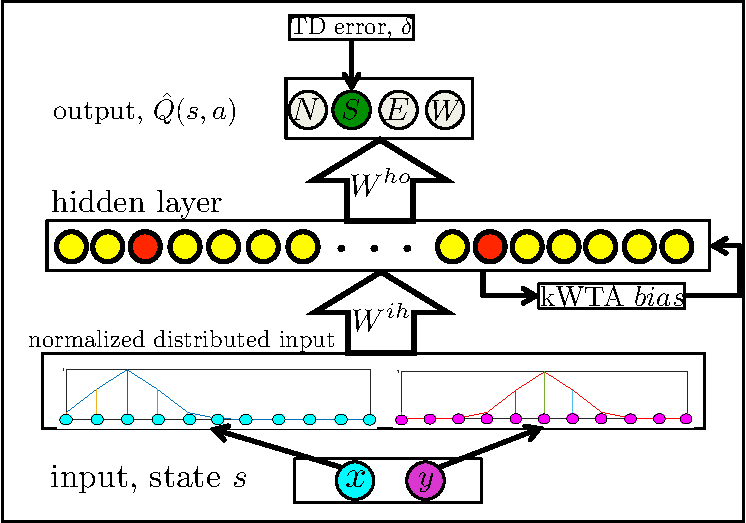
\includegraphics[scale=0.5]{figures/kWTA-schematic.pdf}
\end{center}
\vspace{-4mm}
\caption{All networks had the same input layer and output layer, with
          $42$ input units and $4$ output units for the puddle world task, as an example. The linear network had
          no hidden layer, while the standard backpropagation network
          and the kWTA network had $220$ hidden units. The kWTA network
          produced sparse codes by allowing only $22$ hidden units to
          have non-zero activation at any one time.}
\label{fig:networks}
\end{figure}


% section experimental_design (end)


\section{Simulation Tasks} % (fold)
\label{sec:simulation_tasks}

%Puddle World
	%The Problem - Reward Structure
	%Encoding the State
	%Results - Performance, Value Function, Convergence
\subsection{Puddle World} % (fold)
\label{sub:puddle_world}










For the puddle world task, the $x$-coordinate and the $y$-coordinate
of the current state, $s$, were presented to the neural network over
two separate pools of input units. Note that these coordinate values
were in the range $[0,1]$, as shown in Figure~\ref{puddleworld}. Each
pool of input units consisted of $21$ units, with each unit
corresponding to a coordinate location between $0$ and $1$, inclusive,
in increments of $0.05$. To encode a coordinate value for input to the
network, a Gaussian distribution with a peak value of $1$, a standard
deviation of $0.05$, and a mean equal to the given continuous
coordinate value was used to calculate the activity of each of
the $21$ input units. For example, for a coordinate value
of $0.15$, the input unit corresponding to this value was set to a
maximum activation of $1$ and input units corresponding to coordinate
values above and below $0.15$ were set to activity levels that
decreased with distance from $0.15$ according to the Gaussian
function.

The network had four output units, each corresponding to one of the
four directions of motion. Between the $42$ input units and the $4$
output units was a layer of $220$ hidden units. The hidden layer was
subject to the previously described kWTA mechanism, parameterized so
as to allow $10\%$, or $22$, of the hidden units to be highly active.
The hidden units used a logistic sigmoid activation function on net
input values that were adjusted to allow only $22$ units to be highly
active at any one time. The output units used a linear activation
function (i.e., their activation was equal to their net input). There
was complete connectivity between the input units and the hidden units
and between the hidden units and the output units, with all connection
weights initialized to uniformly sampled random values in the range
$[-0.05,0.05]$.




Following the SARSA version of TD Learning, the reinforcement agent
was controlled in the following way. The current location of the
agent, $s$, was provided as input to the neural network, producing
four output activation values. With a small exploration probability,
$\epsilon$, these values were ignored, and an action was selected
uniformly at random from the four cardinal directions. (The value of
$\epsilon$ is discussed further, below.) Otherwise, the output unit
with the highest activation level determined the action, $a$, to be
taken. The agent then moved a distance of $0.05$ in the direction
specified by the selected action, placing it in a new state, $s'$.



At this point, the agent received a reward signal, $r$, based on its
current location, $s'$. This value was $-1$ for most of the
environment, but it had a higher value, $0$, at the goal location in
the Northeast corner. If the agent was currently located in a puddle,
the reward signal was calculated as $(-400 \times d)$, where $d$ is
the shortest distance from the current location to the edge of the
puddle. Finally, the agent received a reward signal of $-2$ if it had
just attempted to leave the square environment. Thus, the agent was
``punished'' for being anywhere except the goal location, and it was
severely ``punished'' for entering a puddle. This pattern of
reinforcement was selected to parallel that used
in~\citep{SuttonRS:1996:Coarse}.

The action selection process was then repeated at location $s'$,
determining a subsequent action, $a'$. Before this action was taken,
however, the neural network value function approximator had its
connection weights updated according to the SARSA Temporal Difference
(TD) Error:
\[ \delta \ = \ \left( r \ + \ \gamma \ \hat{Q}(s',a') \right) -
   \hat{Q}(s,a) \]
The TD Error, $\delta$, was used to construct an error signal for the
backpropagation network implementing the value function. The network
was given the input corresponding to $s$, and activation was
propagated through the network. Each output unit then received an
error value. This error was set to zero for all output units except
for the unit corresponding to the action that was taken, $a$. The 
selected action unit received an error signal equal to the TD Error,
$\delta$. These error values were then backpropagated through the
network, using the standard backpropagation of error
algorithm~\citep{RumelhartDE:1986:BP}, and connection weights were
updated (with a low learning rate, $\alpha$, of $0.005$). This process
was then begun again, starting at location $s'$ and taking action
$a'$.

The agent explored the puddle world environment in
\emph{episodes}. Each episode began with the agent being placed at a
location within the environment sampled uniformly at random. Actions
were then taken, and connection weights updated, as described
above. The episode ended when the agent reached the goal location or
after the maximum of $80$ actions had been taken. At the beginning of
a simulation, the exploration probability, $\epsilon$, was set to a
relatively high value of $0.1$, and it remained at this value for much
of the learning process. Once the average magnitude of $\delta$ over
an episode fell below $0.2$, the value of $\epsilon$ was reduced by
$0.1\%$ each time the goal location was reached. Thus, as the agent
became increasingly successful at reaching the goal location, the
exploration probability, $\epsilon$, approached zero. (Annealing the
exploration probability is commonly done in systems using TD
Learning.) The agent continued to explore the environment, one episode
after another, until the average absolute value of $\delta$ was below
$0.01$ and the goal location was consistently reached, or a maximum of
$44,100$ episodes had been completed. (This value was heuristically
selected as a function of the size of the environment: $(21 \times 21)
\times 100 = 44,100$.)

When this reinforcement learning process was complete, we examined
both the behavior of the agent and the degree to which its value
function approximations, $\hat{Q}(s,a)$, matched the correct values,
$Q(s,a)$, where the correct values were determined by running SARSA
to convergence while using a large look-up table to capture the value
function.



% subsection puddle_world (end)

%Mountain Car
	% The Problem - Reward Structure
	% Encoding the State
	% Results - Performance, Value Function, Convergence
\subsection{Mountain Car} % (fold)
\label{sub:mountain_car}

The task is dirving a car up to a steep mountain road but the difficulty is that gravity is stronger than car's engine. The agent should learn first to move away goal and use the stored potential energy to convert the kinetic and add full throttle to overcome gravity and reach the goal state. The goal is at the top of the hill at right. 
\begin{figure}
\begin{center}
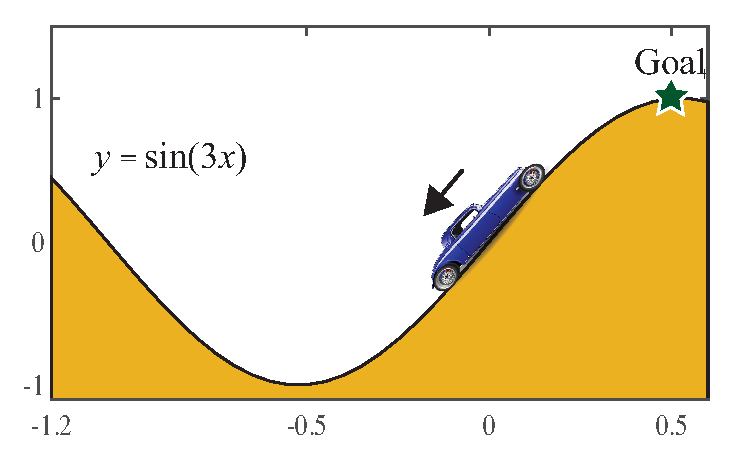
\includegraphics[scale=0.5]{figures/mountainCar-schematic.eps}
\end{center}
\vspace{-4mm}
\caption{The goal is to drive an underpowered car above the steep hill. The agent received -1 reward for each step until it reaches to goal which received 0 reward.}
\label{fig:mountain_car}
\end{figure}

The agent receives reward of -1 for all steps except reaching to goal which reward is 0. The state of mountain car is described by positoin and velocity, $s=(x,\dot{x})$. There are three possible actions: full throttle forward ($a=+1$), zero throttle ($a=0$), full throttle backward ($a=-1$). After choosing action $a$, The car's state is updated by,
\begin{align*}
	x_{t+1} &= \text{bound} (x_t + \dot{x}_{t+1}) \\
	\dot{x}_{t+1} &= \text{bound} (\dot{x}+ 0.0001 a_t - 0.0025 \cos(3 x_t)),
\end{align*}
where bound function keeps state varaibles in their limits, $x \in [-1.2,+0.5]$ and $\dot{x} \in [-0.07,+0.07]$. When the car reaches the left bound, its velocity is reset to zero. Each state variables were devided to uniform meshes. Every episode started from a random position and velocity from descritized state space.  





Both $x$-coordinate and the $\dot{x}$ is uniformly devided to 60 meshes. To encode a state value for input to the
network, a Gaussian distribution with a peak value of $1$, a standard
deviation of $1/60$, and a mean equal to the given continuous
coordinate value was used to calculate the activity of each of
the $61$ input units.

The network had three output units, each corresponding to one of the possible forward, neutral, backward throttle of motor. Between the $122$ input units and the $3$ output units was a layer of $61*61*0.7 = 2604$ hidden units. The hidden layer was
subject to the previously described kWTA mechanism, parameterized so
as to allow $10\%$, or $260$, of the hidden units to be highly active.
The hidden units used a logistic sigmoid activation function on net
input values that were adjusted to allow only $260$ units to be highly
active at any one time. The output units used a linear activation
function (i.e., their activation was equal to their net input). There
was complete connectivity between the input units and the hidden units
and between the hidden units and the output units, with all connection
weights initialized to uniformly sampled random values in the range
$[-0.05,0.05]$.




Following the SARSA version of TD Learning, the reinforcement agent
was controlled in the following way. The current state of the
agent, $s$, was provided as input to the neural network, producing
three output activation values. With a small exploration probability,
$\epsilon$, these values were ignored, and an action was selected
uniformly at random from the four cardinal directions. (The value of
$\epsilon$ is decreseasing from 0.1 to 0.0001 witha rate of 0.99) Otherwise, the output unit
with the highest activation level determined the action, $a$, to be
taken. The state of the agent then updates with by the selected action (Appendix \ref{appen:mountain-car}), placing it in a new state, $s'$.



At this point, the agent received a reward signal, $r$, based on its
current location, $s'$. This value was $-1$ for most of the
environment, but it had a higher value, $0$, at the goal location ($x \geq 0.5$) in
the right side of the hill. When car bumps the boundaries, the velocity is reset to zero, there is no extra punishment for bumping the wall.
The action selection process was then repeated at location $s'$,
determining a subsequent action, $a'$. Before this action was taken,
however, the neural network value function approximator had its
connection weights updated according to the SARSA Temporal Difference
(TD) Error:
\[ \delta \ = \ \left( r \ + \ \gamma \ \hat{Q}(s',a') \right) -
   \hat{Q}(s,a) \]
The TD Error, $\delta$, was used to construct an error signal for the
backpropagation network implementing the value function. The network
was given the input corresponding to $s$, and activation was
propagated through the network. Each output unit then received an
error value. This error was set to zero for all output units except
for the unit corresponding to the action that was taken, $a$. The 
selected action unit received an error signal equal to the TD Error,
$\delta$. These error values were then backpropagated through the
network, using the standard backpropagation of error
algorithm~\citep{RumelhartDE:1986:BP}, and connection weights were
updated (with a low learning rate, $\alpha$, of $0.002$). This process
was then begun again, starting at location $s'$ and taking action
$a'$.

The agent explored the mountain car environment in
\emph{episodes}. Each episode began with the agent being placed at a
location within the environment sampled uniformly at random. Actions
were then taken, and connection weights updated, as described
above. The episode ended when the agent reached the goal location or
after the maximum of $3000$ actions had been taken. At the beginning of
a simulation, the exploration probability, $\epsilon$, was set to a
relatively high value of $0.1$, once the agent reaches the goal, the value of $\epsilon$ was reduced by $0.1\%$ each time the goal location was reached. Thus, as the agent
became increasingly successful at reaching the goal location, the
exploration probability, $\epsilon$, approached to lower bound of 0.0001. (Annealing the
exploration probability is commonly done in systems using TD
Learning.) The agent continued to explore the environment, one episode
after another, until the average absolute value of $\delta$ was below
$0.05$ and the goal location was consistently reached, or a maximum of
$200,000$ episodes had been completed.

When this reinforcement learning process was complete, we examined
both the behavior of the agent and the degree to which its value
function approximations, $\hat{Q}(s,a)$, matched the correct values,
$Q(s,a)$, where the correct values were determined by running SARSA
to convergence while using a large look-up table to capture the value
function.





% subsection mountain_car (end)

\subsection{Acrobot Control Task} % (fold)
\label{sub:acrobot_control_task}
We experimented the hypothesis with Acrobot task which is more complicated and attempted by Suttan \citep{SuttonRS:1996:Coarse}. The \textit{acrobot} is a two-link under-actuated robot, a simple model of a gymnast swinging on a highbar (Figure \ref{fig:acrobot}) \citep{SuttonRS:1996:Coarse}. The state of the acrobot is determined by four continuous state variables; two joint angles $(\theta_1,\theta_2)$ (see figure \ref{fig:acrobot})and corresponding velocities, i.e. $s = (\theta_1,\theta_2,\dot{\theta_1},\dot{\theta_2}).$ The goal is controlling the acrobot to swing until to reach the tip (``feet'') above the bar by an amount of length of the ``hand'' link. The torque is only applied to the second joint. The equations of motion is provided in appendix \ref{appen:acrobot}. The agent receives -1 reward until it reaches to goal which received 0 reward. The frequency of action selection has been set to 5Hz and the time step $\Delta t = 0.05$s is been used for numerical integration of the equations. We used discount factor $\gamma = 0.99$.
\begin{figure}
\begin{center}
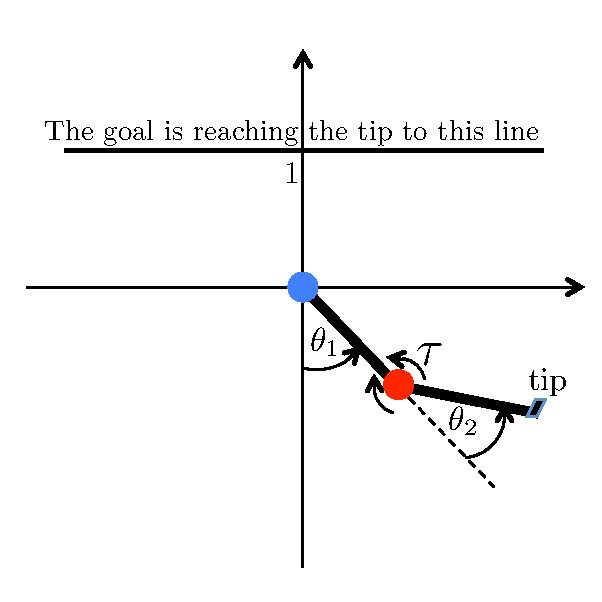
\includegraphics[scale=0.5]{figures/acrobot-schematic.pdf}
\end{center}
\vspace{-4mm}
\caption{The goal is swinging until to reach the tip (``feet'') above the bar by an amount of length of a the ``hand'' link. The agent receives -1 reward until it reaches to goal which received 0 reward.}
\label{fig:acrobot}
\end{figure}

 In our simulation, each of the four dimensions are divided to 20 uniform meshes. To encode a state value for input to the
network, a Gaussian distribution with a peak value of $1$, a standard
deviation of $1/20$, and a mean equal to the given continuous
coordinate value was used to calculate the activity of each of
the $21$ input units.

The network had three output units, each corresponding to one of the possible values of torque applied, clockwise, neutral, counter-clockwise. Between the $84$ input units and the $3$ output units was a layer of $8400$ hidden units for kWTA networks and $19448$ for regular backpropagation network. The hidden layer was
subject to the previously described kWTA mechanism, parameterized so
as to allow $10\%$, or $840$, of the hidden units to be highly active.
The hidden units used a logistic sigmoid activation function on net
input values that were adjusted to allow only $840$ units to be highly
active at any one time. The output units used a linear activation
function (i.e., their activation was equal to their net input). There
was complete connectivity between the input units and the hidden units
and between the hidden units and the output units, with all connection
weights initialized to uniformly sampled random values in the range
$[-0.05,0.05]$.




Following the SARSA version of TD Learning, the reinforcement agent
was controlled in the following way. The current state of the
agent, $s$, was provided as input to the neural network, producing
three output activation values. With a small exploration probability,
$\epsilon$, these values were ignored, and an action was selected
uniformly at random from the four cardinal directions. (The value of
$\epsilon$ is decreseasing from 0.05 to 0.0001 witha rate of 0.99) Otherwise, the output unit
with the highest activation level determined the action, $a$, to be
taken. The state of the agent then updates with by the selected action (Appendix \ref{appen:acrobot}), placing it in a new state, $s'$.



At this point, the agent received a reward signal, $r$, based on its
current state, $s'$. This value was $-1$ for most of the
environment, but it had a higher value, $0$, at the goal location ($y_{tip} \geq 1$). The action selection process was then repeated at location $s'$,
determining a subsequent action, $a'$. Before this action was taken,
however, the neural network value function approximator had its
connection weights updated according to the SARSA Temporal Difference
(TD) Error:
\[ \delta \ = \ \left( r \ + \ \gamma \ \hat{Q}(s',a') \right) -
   \hat{Q}(s,a) \]
The TD Error, $\delta$, was used to construct an error signal for the
backpropagation network implementing the value function. The network
was given the input corresponding to $s$, and activation was
propagated through the network. Each output unit then received an
error value. This error was set to zero for all output units except
for the unit corresponding to the action that was taken, $a$. The 
selected action unit received an error signal equal to the TD Error,
$\delta$. These error values were then backpropagated through the
network, using the standard backpropagation of error
algorithm~\citep{RumelhartDE:1986:BP}, and connection weights were
updated (with a low learning rate, $\alpha$, of $0.002$). This process
was then begun again, starting at location $s'$ and taking action
$a'$.

The acrobot agent explored environment in
\emph{episodes}. Each episodes of learning starts with the acrobot agant hanging straight down and at rest i.e. $s=(0,0,0,0)$. Actions
were then taken, and connection weights updated, as described
above. The episode ended when the agent reached the goal location or
after the maximum of $2000$ actions had been taken. At the beginning of
a simulation, the exploration probability, $\epsilon$, was set to a
relatively high value of $0.05$, once the agent reaches the goal, the value of $\epsilon$ was reduced by $0.1\%$ each time the goal location was reached. Thus, as the agent
became increasingly successful at reaching the goal location, the
exploration probability, $\epsilon$, approached to lower bound of 0.0001. (Annealing the
exploration probability is commonly done in systems using TD
Learning.) The agent continued to explore the environment, one episode
after another, until the average absolute value of $\delta$ was below
$0.05$ and the goal location was consistently reached, or a maximum of
$200,000$ episodes had been completed.

When this reinforcement learning process was complete, we examined
both the behavior of the agent and the degree to which its value
function approximations, $\hat{Q}(s,a)$, matched the correct values,
$Q(s,a)$, where the correct values were determined by running SARSA
to convergence while using a large look-up table to capture the value
function.




%% Acrobat
% The Problem - Reward Structure
% Encoding the State
% Results - Performance, Value Function, Convergence

% subsection acrobot_control_task (end) 

% section simulation_tasks (end)

\section{Simulation Results} % (fold)
\label{sec:simulation_results}

We compared the performance of our kWTA neural network with that
produced by using a standard backpropagation network with identical
parameters. We also examined the performance of a ``linear'' network,
which had no hidden units but only complete connections from all input
units directly to the four output units.


\subsection{Puddle World Task}
\label{sub:puddle_world_results}


\begin{figure*}[t]
\begin{center}
\begin{tabular}[h]{ccc}
\raisebox{5mm}{Linear}  & \raisebox{5mm}{BP} &  \raisebox{5mm}{kWTA} \\ 
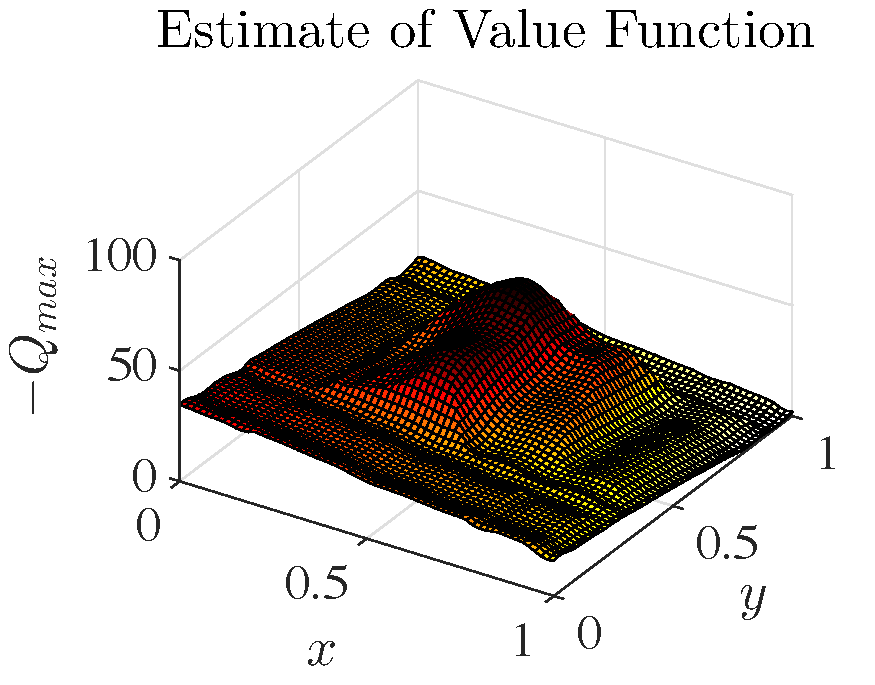
\includegraphics[scale=0.30]{figures/puddleWorld-linear-value.pdf}   &
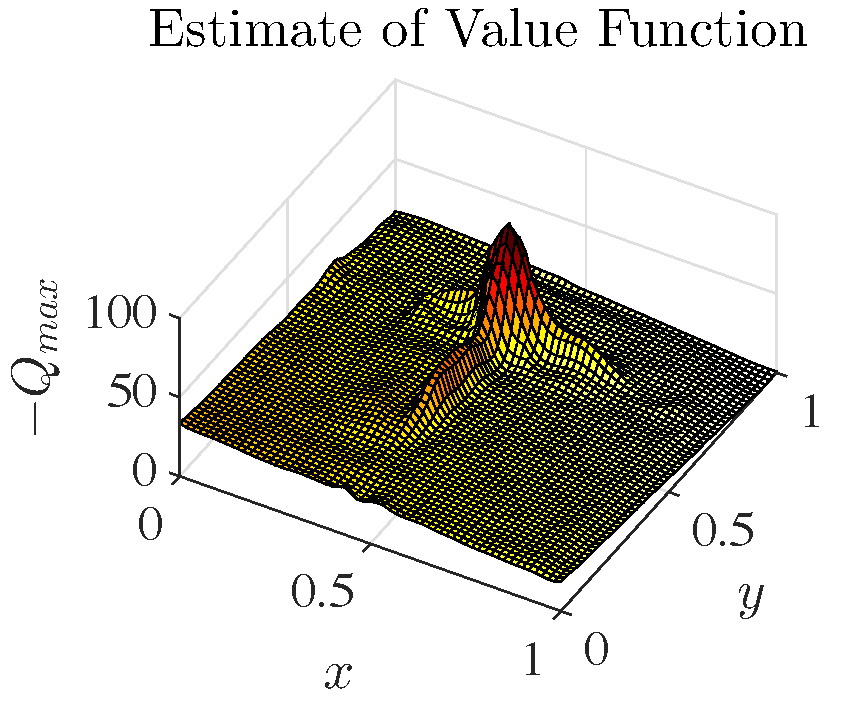
\includegraphics[scale=0.30]{figures/puddleWorld-bp-value.pdf}       &
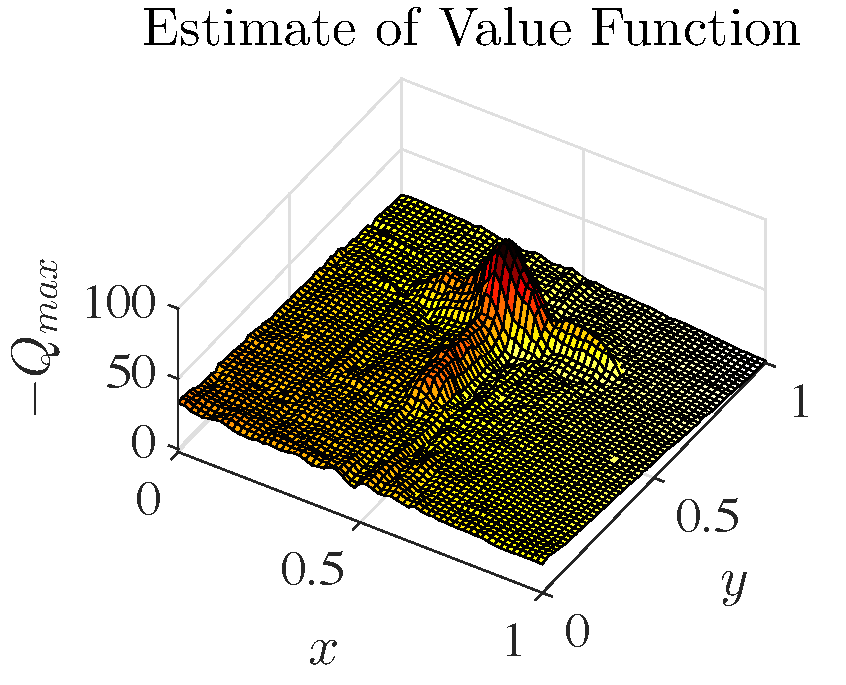
\includegraphics[scale=0.30]{figures/puddleWorld-kwta-value.pdf}     \\
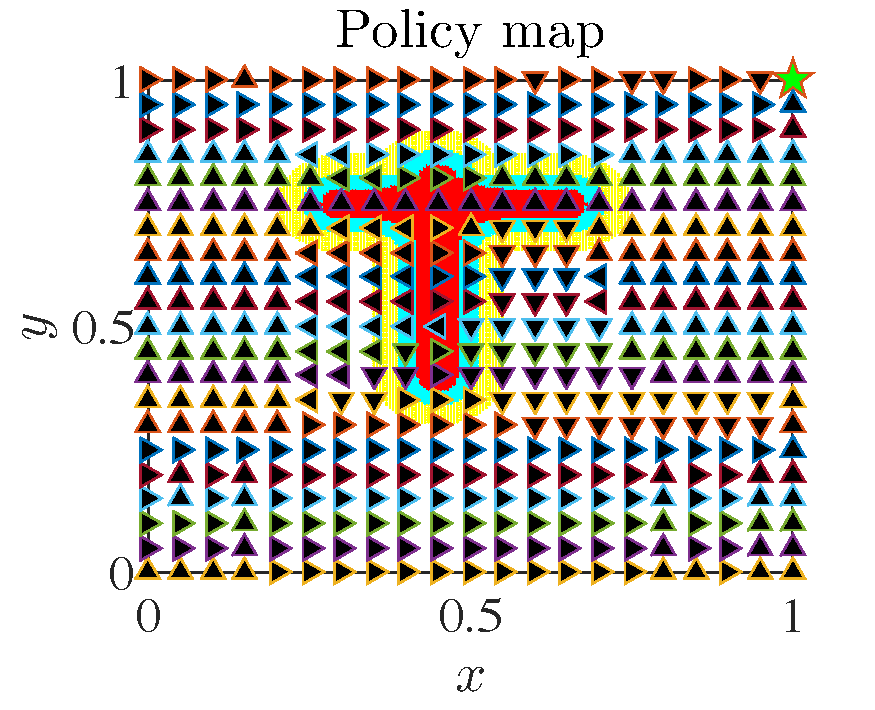
\includegraphics[scale=0.30]{figures/puddleWorld-linear-policy.pdf}  &
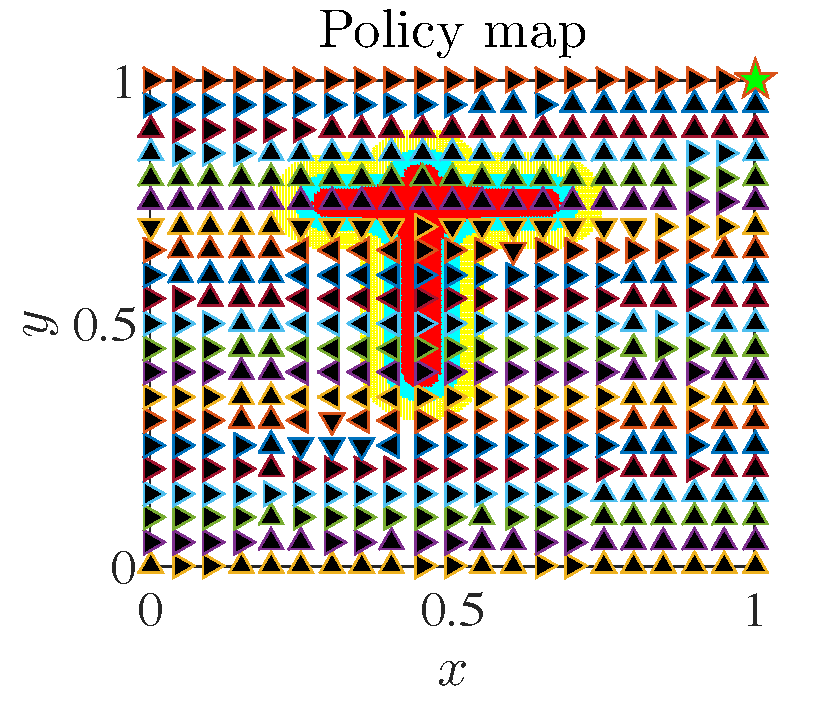
\includegraphics[scale=0.30]{figures/puddleWorld-bp-policy.pdf}      &
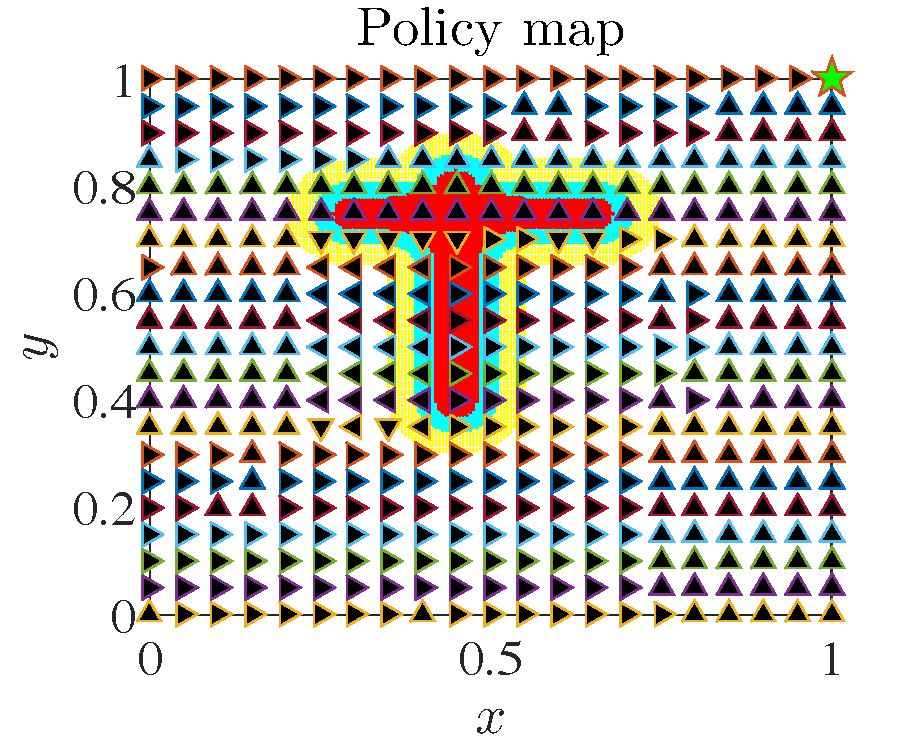
\includegraphics[scale=0.30]{figures/puddleWorld-kwta-policy.pdf}    \\
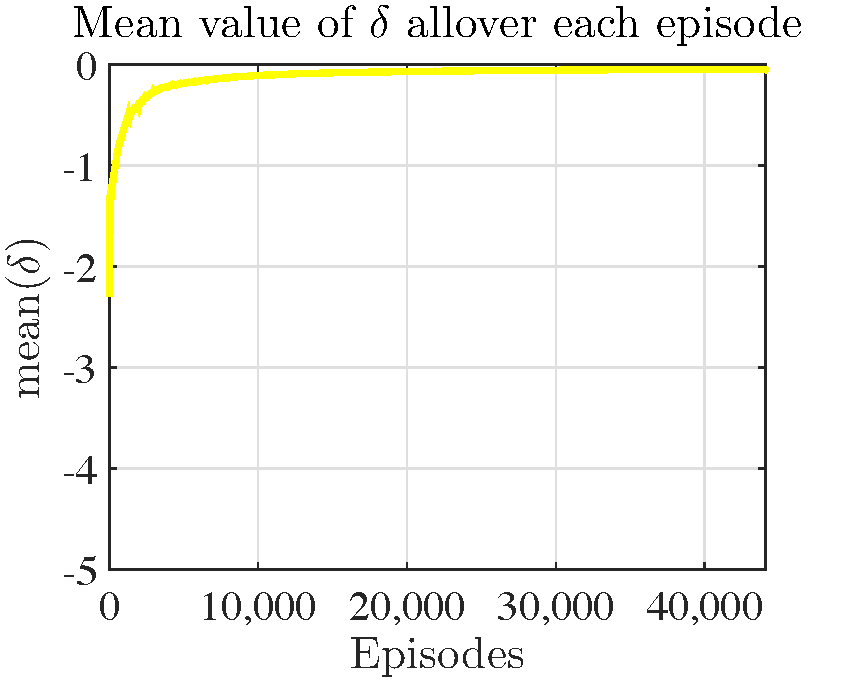
\includegraphics[scale=0.30]{figures/puddleWorld-linear-delta.pdf}   &
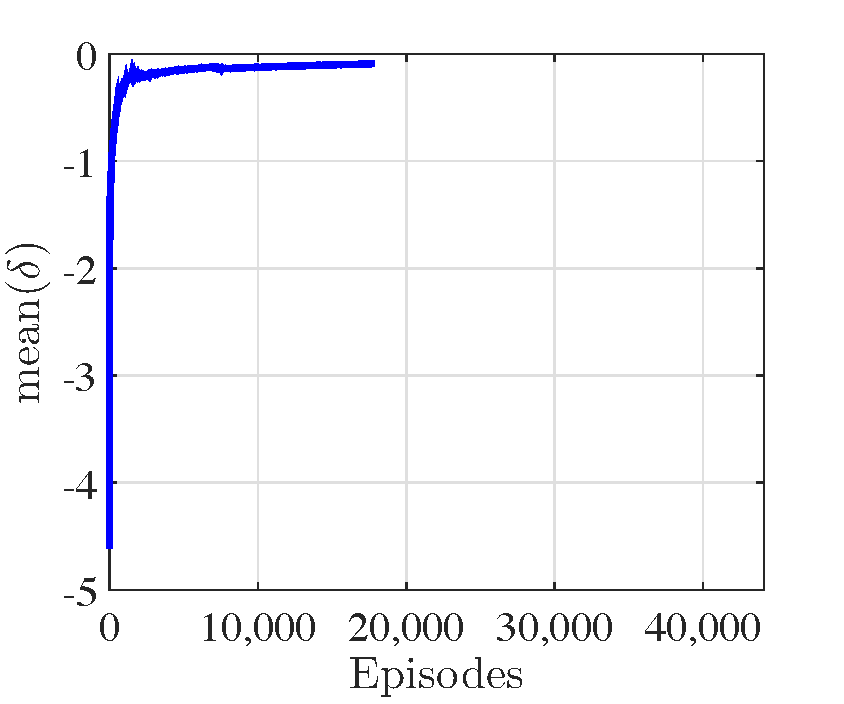
\includegraphics[scale=0.30]{figures/puddleWorld-bp-delta.pdf}       &
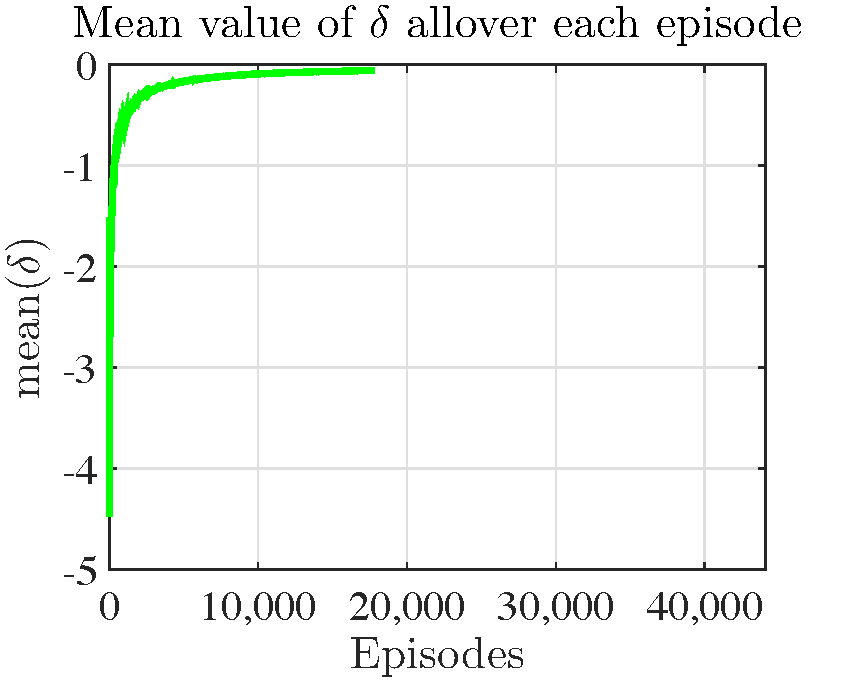
\includegraphics[scale=0.30]{figures/puddleWorld-kwta-delta.pdf}
\end{tabular}
\end{center}
\caption{The performance of various learned value function
         approximators may be compared in terms of their success at
         learning the true value function, the resulting action
         selection policy, and the amount of experience in the
         environment needed to learn. The approximated value
         functions, expressed as $\mbox{\it max}_{a}\ \hat{Q}(s,a)$
         for each location, $s$, appears on the left. The actions
         selected at a grid of locations is shown in the middle
         column. The learning curve, showing the TD Error over
         learning episodes, is shown on the right. The rows display
         results for representative neural networks of the three kinds
         explored:  linear, backpropagation, and kWTA, respectively,
         from top to bottom.}
\label{bigresults}
\end{figure*}



\subsection{Mountain Car Task} % (fold)
\label{sub:mountain_car_results}


\begin{figure*}
\begin{center}
\begin{tabular}[h]{ccc}
\raisebox{10mm}{Linear} & \raisebox{10mm}{BP}  & \raisebox{10mm}{kWTA} \\
\includegraphics[scale=0.2]{figures/mountainCar-linearNN-cost.eps} &
\includegraphics[scale=0.2]{figures/mountainCar-regularBPNN-cost.eps} & 
\includegraphics[scale=0.2]{figures/mountainCar-kwtaNN-cost.eps} \\
\includegraphics[scale=0.2]{figures/mountainCar-linearNN-performance.eps} &
\includegraphics[scale=0.2]{figures/mountainCar-regularBPNN-performance.eps} & 
\includegraphics[scale=0.2]{figures/mountainCar-kwtaNN-performance.eps} \\
\includegraphics[scale=0.2]{figures/mountainCar-linearNN-frozen-test.eps}  &
\includegraphics[scale=0.2]{figures/mountainCar-regularBPNN-frozen-test.eps} &
\includegraphics[scale=0.2]{figures/mountainCar-kwtaNN-frozen-test.eps}    
\end{tabular}
\end{center}
\caption{The performance of various networks trained for mountain car.} 
\label{bigresults}
\end{figure*}



% subsection mountain_car_results (end)

% section simulation_results (end)


\subsection{Acrobot Task}
\label{sub:acrobot_results}

\begin{figure*}
\begin{center}
\begin{tabular}[h]{ccc}
\raisebox{10mm}{Linear} & \raisebox{10mm}{BP}  & \raisebox{10mm}{kWTA} \\
\includegraphics[scale=0.2]{figures/acrobot-linearNN-performance.eps}  &
\includegraphics[scale=0.2]{figures/acrobot-regularBPNN-performance.eps} &
\includegraphics[scale=0.2]{figures/acrobot-kwtaNN-performance.eps} \\
\includegraphics[scale=0.2]{figures/acrobot-linearNN-frozen-test.eps} &
\includegraphics[scale=0.2]{figures/acrobot-regularBPNN-frozen-test.eps} &
\includegraphics[scale=0.2]{figures/acrobot-kwtaNN-frozen-test.eps} 
\end{tabular}
\end{center}
\caption{The Acrobot task performance.}
\label{bigresults}
\end{figure*}


\section{Discussion}

\section{Conclusion}



%% The Appendices part is started with the command \appendix;
%% appendix sections are then done as normal sections
 \appendix

 \section{acrobot}
 \label{appen:acrobot}
The equations of motion for acrobot are,
\begin{gather*}
\ddot{\theta_1} = -d_1^{-1} (d_2 \ddot{\theta_2} + \phi_2),\\
\ddot{\theta_2} = - \left( m_2 l^{2}_{c2} + I_2 - \frac{d^{2}_2}{d_1} \right)^{-1} \left( \tau + \frac{d_2}{d_1} \phi_1 - \phi_2 \right), 
\end{gather*}
\begin{gather*}
d_1 = m_1 l^{2}_{c1} + m_2 l_1 l_{c2} \cos(\theta_2) + I_2,  \\
d_2 = m_2 \left( l_{c2}^{2} + l_1 l_{c2} \cos(\theta_2) \right) + I_2, 
\end{gather*}
\begin{gather*}
\phi_1 = - m_2 l_1 l_{c2} \dot{\theta_1}^2 \sin(\theta_2) - 2 m_2 l_1 l_{c2} \dot{\theta_2} \dot{\theta_1}\sin(\theta_2) + (m_1 l_{c1} + m_2 l_{1})g \cos(\theta_1 - \pi / 2) + \phi_2,  \\
\phi_2 = m_2 l_{c2}g \cos(\theta_1 + \theta_2 - \pi / 2).
\end{gather*}

The torque $\tau \in \{-1,0,1\}$ which is only applied to the second joint. The angular velocities are bounded to $\theta_1 \in [-4\pi,4\pi]$ and $\theta_2 \in [-9 \pi, 9\pi]$. The $m_1=1$ and $m_2=1$ are the masses of the links and $l_1 = 1 m$ and $l_2 = 1 m$ are the lengths of the links. $l_{c1}=l_{c1}=0.5 m$ are the lenghts of center of mass of links, $I_1 = I_2 = 1 kg.m^2$ are the moments of inertia of links, $g = 9.8 m/s^2$ is the constant of gravity.   






\section{algorithm}
%% put codes on git hub
\label{appen:algorithm}



\section{mountain car}
\label{appen:mountain-car}

\section{puddle world}
\label{appen:puddle-world}




%%
%% \bibliographystyle{elsarticle-num-names}
\bibliographystyle{elsarticle-harv}
\bibliography{BICA}


\end{document}
\endinput